\documentclass[11pt]{article}
\usepackage[margin=1in]{geometry}
\usepackage{graphicx,booktabs,amsmath}
\usepackage[colorlinks=true,urlcolor=blue,linkcolor=blue]{hyperref}
\usepackage{enumitem}
\title{Arithmetic, Answer Formatting, and Generalization\\in a Tiny Language Model Trained with GRPO}
\author{Mohamed Sobhy}
\date{Living experiment report --- October 2026}
\begin{document}
\maketitle
\begin{abstract}
This project investigates direct reinforcement learning on a pretrained
0.8-billion-parameter language model for Countdown arithmetic. A pilot run
improved strict greedy accuracy from 0/256 to 85/256 (33.2\%) on a fixed held-out
set after 300 optimizer steps. This report distinguishes measured findings from
planned experiments. A post-hoc audit using a conservative declared-expression
parser recovers the same correct counts when the answer-tag requirement is
relaxed. This supports investigating arithmetic task improvement, while not
establishing general reasoning or fully identifying the role of formatting.
Output-budget, multi-seed, reward-ablation, and distribution-shift experiments
are tracked below as they are completed.
\end{abstract}

\section{Question and experimental scope}
When does direct GRPO improve arithmetic task performance, and how much of an
apparent improvement is answer-format compliance? The base checkpoint is
\texttt{Qwen/Qwen3.5-0.8B-Base}; the dataset is
\texttt{Jiayi-Pan/Countdown-Tasks-3to4}. The experiment omits supervised
fine-tuning. It does not train a model from scratch and does not claim discovery
of general reasoning. Model and dataset revisions, code, and outputs are retained
in the \href{https://github.com/mohamedsobhi777/countdown-grpo}{public repository}.

\section{Pilot protocol}
The text backbone is trained with BF16 rank-16 LoRA on one RTX 4090 Laptop GPU
with 16 GB VRAM. GRPO uses eight candidates per puzzle, 32 completions per
optimizer step, a learning rate of $10^{-5}$, no KL penalty, and a 256-token
completion limit. The 300-step run used seed 42 and took 5,135.9 seconds of
training time (85.6 minutes), excluding setup and evaluation.

Puzzles are deduplicated by $(\text{target},\operatorname{sort}(\text{numbers}))$.
A seeded hash partition reserves 2\% for evaluation before subset selection.
The available training subset contains 20,000 puzzles; evaluation uses 256 fixed
puzzles. Both base and adapter evaluations use greedy decoding with the same
output limit. No evaluation-based checkpoint selection was performed.

The strict reward is binary: one final \texttt{<answer>} block must contain a
valid arithmetic expression using each supplied number exactly once. The
verifier supports binary $+, -, \times, /$, parentheses, and exact rational
arithmetic. It rejects number reuse/omission and unsafe syntax. Negative and
fractional intermediate values are allowed. No formatting bonus was used.

\section{Pilot results}
\begin{center}
\begin{tabular}{lrr}
\toprule
Metric on 256 held-out puzzles & Base & GRPO adapter\\
\midrule
Strict correct & 0 (0.0\%) & 85 (33.2\%)\\
Strict valid expressions & 11 (4.3\%) & 90 (35.2\%)\\
Declared-expression diagnostic correct & 0 (0.0\%) & 85 (33.2\%)\\
\bottomrule
\end{tabular}
\end{center}
\begin{figure}[ht]
\centering
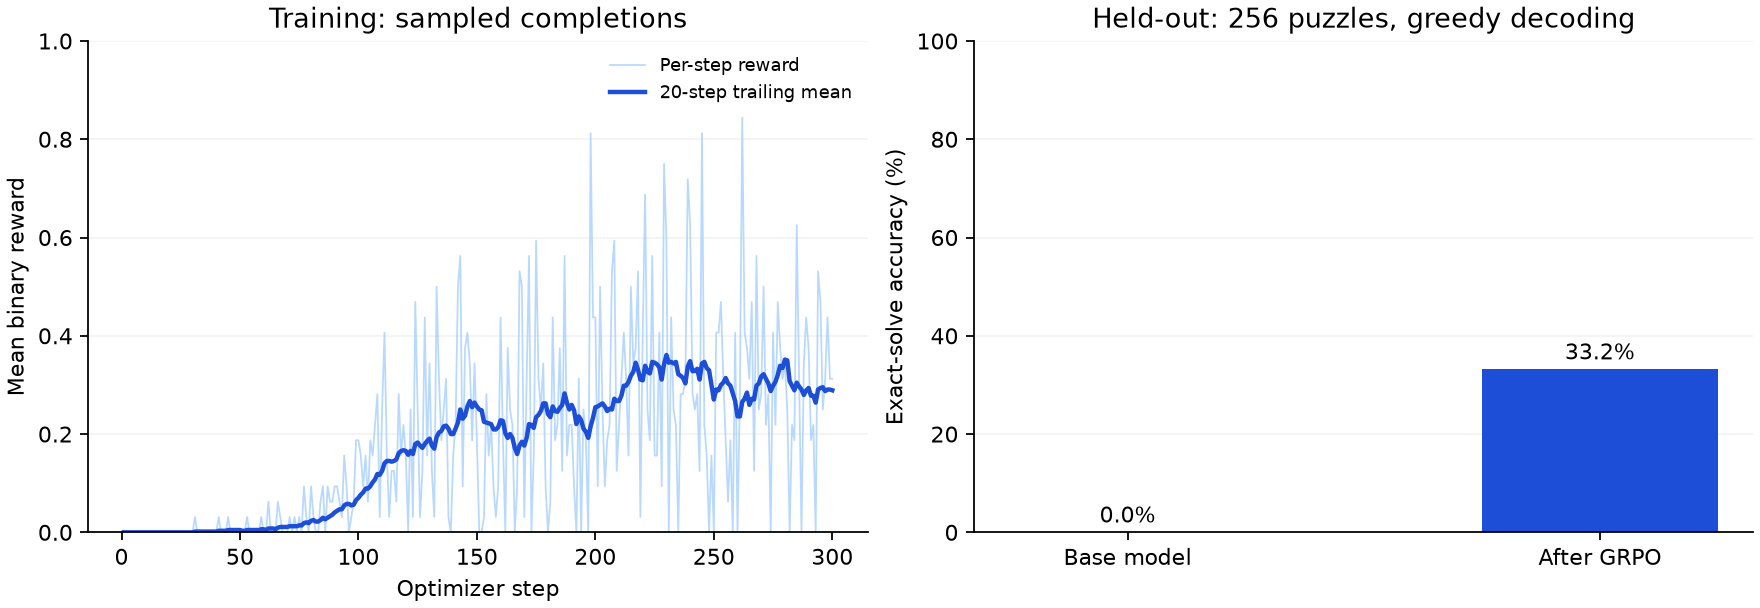
\includegraphics[width=\linewidth]{figures/pilot.png}
\caption{Pilot stochastic training reward and separate greedy held-out accuracy.
These use different puzzles and decoding protocols; validation was not measured
at every training step.}
\end{figure}
The first positive training reward occurred at step 31. Peak PyTorch-allocated
memory was 2.72 GiB, which excludes reserved memory and other GPU allocations.
In the final 30 training steps, 59.9\% of sampled completions reached the output
cap. Historical evaluation reports do not record termination token IDs, so their
truncation status is unknown rather than inferred from decoded text.

\section{Format-independent diagnostic: declared-expression-v1}
This diagnostic is post-hoc and is not used as a training reward. Extraction is
deterministic and independent of the target:
\begin{enumerate}[nosep]
\item If answer tags occur, require exactly one complete block and extract it.
      A wrong tagged answer never falls back to an earlier expression.
\item Otherwise, select the last standalone arithmetic line, allowing an
      optional ``Answer:'' or ``Final answer:'' prefix and simple math/code delimiters.
\item For an equation, evaluate only the leftmost expression. Do not trust its
      claimed right-hand value or search intermediate calculations for a success.
\item Apply bounded AST interpretation, exact rational evaluation, and multiset
      validation of input numbers. Reject unsupported operations and syntax.
\end{enumerate}
This conservative parser can miss correct answers expressed in prose or other
notation. Therefore equal strict and diagnostic counts do not prove formatting
had no causal role in training. They show that this specified relaxation did not
recover additional correct answers from the archived generations.

\begin{center}
\begin{tabular}{lrr}
\toprule
Diagnostic outcome & Base & Adapter\\
\midrule
Correct & 0 & 85\\
Wrong numerical value with valid numbers & 90 & 5\\
Number multiset mismatch & 152 & 121\\
Invalid syntax & 10 & 19\\
No declared expression & 4 & 24\\
Ambiguous or incomplete answer tags & 0 & 2\\
\bottomrule
\end{tabular}
\end{center}
These are mutually exclusive diagnostic categories. Number omission/reuse details
are retained per answer; truncation is a separate flag when token metadata exists.
All 512 historical outputs were re-scored, and strict scores matched their
original records. The same unique holdout puzzles were verified in both reports,
with no intersection with the selected training subset.
An independent exact subset-dynamic-programming solver found a valid witness for
all 256 puzzles under the all-inputs-once rules. Unsolvable holdout items therefore
do not explain the errors. Witnesses are archived separately and never included
in model prompts. An agent review of the first two records per observed outcome
category (20 records total) found agreement with the specified extraction rule;
this is not a blinded human annotation study. Prose-heavy and incomplete outputs
illustrate the parser's coverage limitations.

\section{Controlled study design and current status}
The study keeps the original strict metric alongside the diagnostic. Planned
comparisons are not presented as completed results:
\begin{itemize}[nosep]
\item Matched base/adapter output budgets of 256, 512, and 1024 tokens; record actual
      generated lengths, EOS status, truncation, and generation time.
\item Binary correctness versus a 0.05 bonus for valid incorrect expressions,
      with training seeds 42, 43, and 44 and a fixed split seed of 42.
\item Three-number-only training with disjoint three- and four-number evaluation.
\item Separately labeled, deterministic, solver-verified suites with larger
      inputs and out-of-range targets; solutions are never included in prompts.
\item A comparison demo with exact verifier feedback and archived examples.
\end{itemize}
Per-seed results and held-out uncertainty will be reported separately. Four
distribution-shift/arity suites have been frozen before querying trained models.

\paragraph{Uncertainty and paired analysis.} Individual checkpoint accuracies use
95\% Wilson score intervals, following the
\href{https://www.itl.nist.gov/div898/handbook/prc/section2/prc241.htm}{NIST formulation}.
For the pilot's 85/256 score this interval is 27.7--39.2\%. It describes
puzzle-sampling uncertainty under a binomial model, not training-seed variability
or uncertainty about arbitrary out-of-distribution tasks. Comparisons match
canonical puzzles and report gained, lost, jointly correct, and jointly incorrect
answers. Exact two-sided McNemar tests are exploratory, with unadjusted p-values;
we do not use the grid to claim a confirmatory significance result.
The controlled-study aggregator requires all six runs to finish and checks
their full training configuration, all 300 optimizer-step records, 20,000 unique
training puzzles, identical ordered train/holdout lists, absence of overlap,
adapter paths, and recomputed evaluation scores. It reports per-seed accuracies
and sample standard deviations, together with paired reward differences for each
seed. Repeated evaluation of the same holdout is not pooled into 768 independent
puzzles. Synthetic manifest tests reject unfinished runs and altered scores;
the complete CPU suite now contains 41 passing tests. Hardware/package equality
must additionally be checked in the linked W\&B provenance before final claims.

\paragraph{Partial output-budget result.} The trained adapter solved 86/256
puzzles at 512 tokens, compared with 85/256 at 256 tokens: one gained solution
and no lost solutions. At 512 tokens, 140/256 outputs (54.7\%) still hit the cap.
Strict and diagnostic scores coincide. The
\href{https://wandb.ai/mohamedsobhi777/countdown-grpo/runs/vnvj9eez}{512-token evaluation}
therefore provides little evidence that doubling the output budget resolves the
pilot's failures. The 1024-token cells are still pending; this is not the final
budget comparison.

\section{Interactive comparison demo}
A local browser interface exposes all 256 archived evaluation pairs, including
failures, with filters for outcomes and number-multiset errors. An exact answer
checker accepts user expressions and shows strict success, diagnostic success,
the extracted expression, exact value, and missing or reused inputs. Archived
mode uses only Python's standard library and requires no model download or GPU.
An optional live mode loads the pilot LoRA adapter and compares greedy generation
with the adapter enabled and disabled; its GPU smoke test remains pending.
The server binds to loopback and serializes live inference requests.

Chromium checks verified all 256 examples, 85-success/171-failure filtering,
interactive answer checking, disabled generation in archived mode, no JavaScript
errors, and mobile layout without horizontal overflow at 390px width. HTTP tests
also check invalid inputs and cross-origin request rejection. All 40 CPU tests
pass. Browser checks are reproducible with
\texttt{scripts/check\_demo\_browser.py}; these do not substitute for testing live
model inference. Single-puzzle generation can differ from the historical batched
evaluation, and custom puzzles are not guaranteed solvable.

\section{Provenance and experiment ledger}
The pilot used clean source commit
\texttt{0a432a272591f7683b711a9c867c01e7d939fca1}. W\&B contains source snapshots,
configs, package versions, puzzle splits, checkpoints, and generation tables:
\begin{itemize}[nosep]
\item \href{https://wandb.ai/mohamedsobhi777/countdown-grpo/runs/qu1ovu2z}{Pilot baseline}
\item \href{https://wandb.ai/mohamedsobhi777/countdown-grpo/runs/uv3hjjih}{Pilot training}
\item \href{https://wandb.ai/mohamedsobhi777/countdown-grpo/runs/1qrixzrf}{Pilot final evaluation}
\item \href{https://wandb.ai/mohamedsobhi777/countdown-grpo/artifacts/model/uv3hjjih-adapter/v0}{Final pilot adapter artifact}
\item \href{https://wandb.ai/mohamedsobhi777/countdown-grpo/workspace}{Study workspace}
\item \href{https://wandb.ai/mohamedsobhi777/countdown-grpo/runs/jyyk55pq}{Archived-output diagnostic audit}
\end{itemize}
\paragraph{2026-10-10.} Inspected the current repository, pilot artifacts, local GPU,
and Overleaf access. Recorded the approved research plan. Implemented and tested
the declared-expression diagnostic, re-scored archived outputs, and added token
termination metadata and output-budget overrides to evaluation. Twenty-five CPU
tests initially passed; solver coverage increased this to 29 tests. Created and
compiled this Overleaf report, verified all holdout puzzles are solvable, and
reviewed a deterministic diagnostic sample. The matched output-budget grid is
running. Six controlled training runs are queued on a Colab L4; the first is
live. Its initial five steps averaged approximately 50.5 seconds per step using
the reference PyTorch attention implementation. These are preliminary throughput
measurements, not a completed training runtime. Statistical analysis and pairing
validation bring CPU coverage to 36 passing tests.

\section{Limitations}
One seed and 256 puzzles do not establish robust generalization. Training-dataset
deduplication cannot rule out exposure in pretraining. Strict success conflates
arithmetic correctness with protocol compliance; the diagnostic is an imperfect
post-hoc measure, not a causal decomposition. Long answers may contain useful
work but still fail due to truncation. No cross-seed, longer-output, or OOD claims
are made until the corresponding experiments finish.
\end{document}
